%
% Catam project simulating wind forced ocean currents
%
\documentclass{article}
\usepackage{amsmath}
\usepackage{empheq}
\usepackage{graphicx}
\usepackage{bm}
\usepackage{framed}
%\usepackage{epstopdf}
%\usepackage{color}
%\usepackage{pgfplots}
\usepackage{caption}
\usepackage{amsfonts}
\usepackage[margin=3cm]{geometry}
\usepackage{float}

\begin{document}

\title{Dynamical Systems}
\author{Dominic Skinner}
\maketitle
\section*{Introduction}
A dynamical system is a set of equations describing the evolution of a system
with respect to a time-like variable. Usually they are non-linear.
\\
The possible states of the system define the state space/phase space.
\\
\\
\textbf{Example:}   The logistic map
\[ x_{n+1} = \mu x_n ( 1- x_n) \]
For $ 0 \leq \mu \leq 4 $ this describes evolution with respect to a discrete time 
$n$ in a state space $[0,1]$.
\\
\\
\textbf{Example:}   The Lotka-Voltera equations
\begin{align*}
\dot{r} &= r(a - br -cs) \\
\dot{s} &= s(d - er -fs)
\end{align*}
Where \emph{a-f} are positive constants. These describe continous evolution 
in a state space $(r,s) \in [0 , \infty] \times [0, \infty]$ as a model for 
the population of two species competing for the same food supply.
\\
\\
\textbf{Example:}   The non-linear Schr\"odinger equation
\[ i \frac{\partial \Psi}{ \partial t} = \nabla^2 \Psi + |\Psi|^2 \Psi \]
This describes evolution in an infinite dimensional statespace of possible
wavefunctions.
\\
\\
Because the equations are non-linear, it is often impossible to find a complete
set of closed form analytic solutions. Instead, we resort to a mixture of 
geometric and analytic arguments, and aim to say something about the generic
long-term behaviour.
\\
\\
\textbf{Example:}   
\begin{align*}
\dot{r} &= r(3 - r -s) \\
\dot{s} &= s(2 - r -s)
\end{align*}
Consider the regions where $\dot{r}$ and $\dot{s}$ are $>0, \; <0, \; =0$. 
\\
If $r,s >0$ then
\begin{align*}
r+s &< 2 \implies \dot{r}, \dot{s} > 0 \\
2 < r+s &< 3 \implies \dot{r} >0 , \; \dot{s} < 0 \\
r+s &> 3 \implies \dot{r}, \dot{s} < 0 \\
\end{align*}
$\dot{r} = 0$ if $r=0$ or $r+s = 3$. \\
$\dot{s} = 0$ if $s=0$ or $r+s = 2$. \\
Therefore $\dot{r} = \dot{s} = 0$ at the fixed points $(0,0), \; (3,0), \; (0,2)$.
This gives the phase portrait/diagram/plane%
\footnote{Phase portrait, phase diagram, phase plane will be used interchangably}
% INCLUDE GRAPHIS HERE
\begin{figure}[H]
\centering
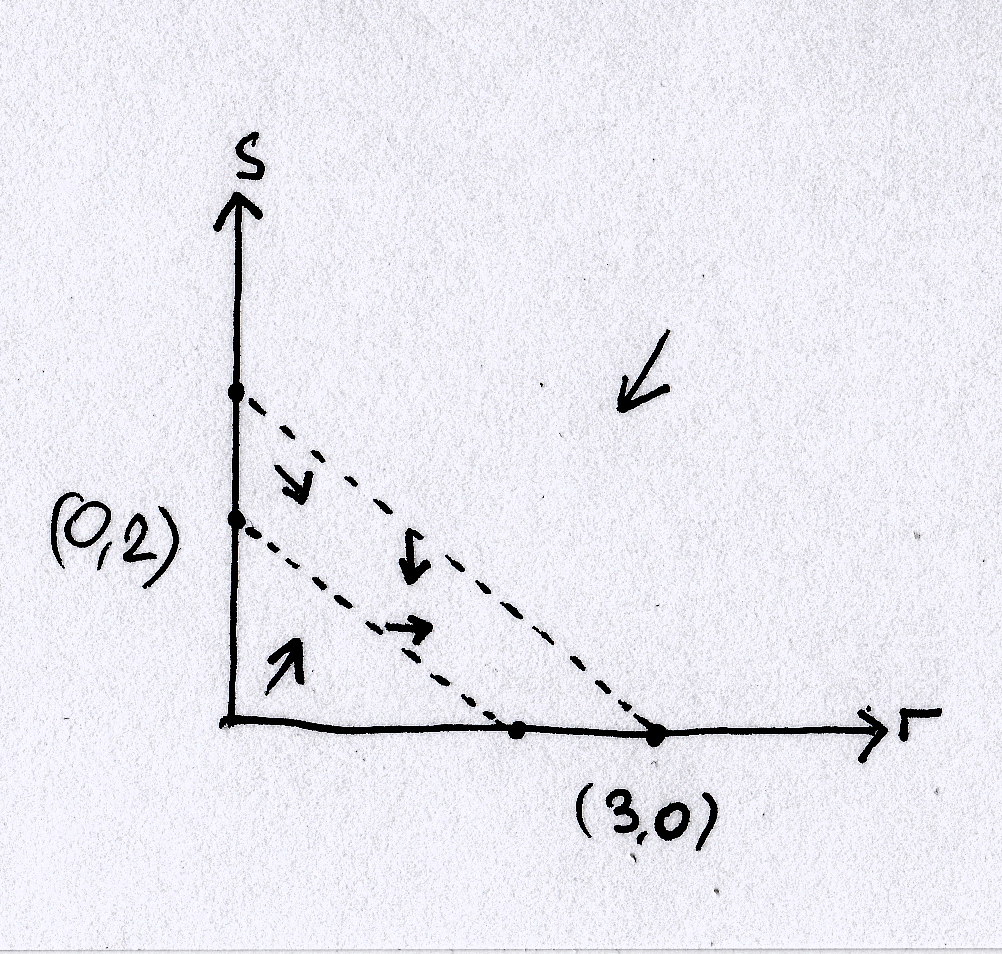
\includegraphics[width=4cm, height=4cm]{fig0.png}
\end{figure}
The most important feature of the phase portrait is that all solutions with 
$r >0$ tend to the stable fixed point $(3,0)$. The fixed points $(0,0)$ and
$(0,2)$ are unstable. There are no periodic orbits.
\\
\\
\textbf{Example:}   
\begin{align*}
\dot{r} &= r(3 - r -s) \\
\dot{s} &= s(2 - \mu r -s)
\end{align*}
In this case, a new fixed point $(\frac{1}{1- \mu} , \frac{2 - 3 \mu}{1- \mu})$
appears in the state space at $\mu = \frac{2}{3}$ and for $\mu < \frac{2}{3}$ 
is the long term stable attractor. 
\\
A qualitative change in the solution structure is called a bifurcation.
\\
\\
\textbf{Example:}   
\begin{align*}
\dot{x} &= -y + \epsilon x (\mu - x^2 - y^2) \\
\dot{y} &= \;\;\; x + \epsilon y (\mu - x^2 - y^2)
\end{align*}
Use polar coordinates which are a more natural choice for this problem.
In general:
\begin{empheq}[box=\fbox]{align}
\dot{r} &= \frac{x \dot{x} + y \dot{y}}{r} \nonumber \\
\dot{\theta} &= \frac{x \dot{y} - y \dot{x} }{ r^2} \nonumber
\end{empheq}
Which are equations that will be referred to frequently. \footnote{so learn them now!}
In our example, they become
\begin{align*}
\dot{r} &= \epsilon r (\mu - r^2) \\
\dot{\theta} &= 1
\end{align*}
Consider $\dot{r}$ and $\dot{\theta}$:
% INSERT DIAGRAM HERE
\begin{figure}[H]
\centering
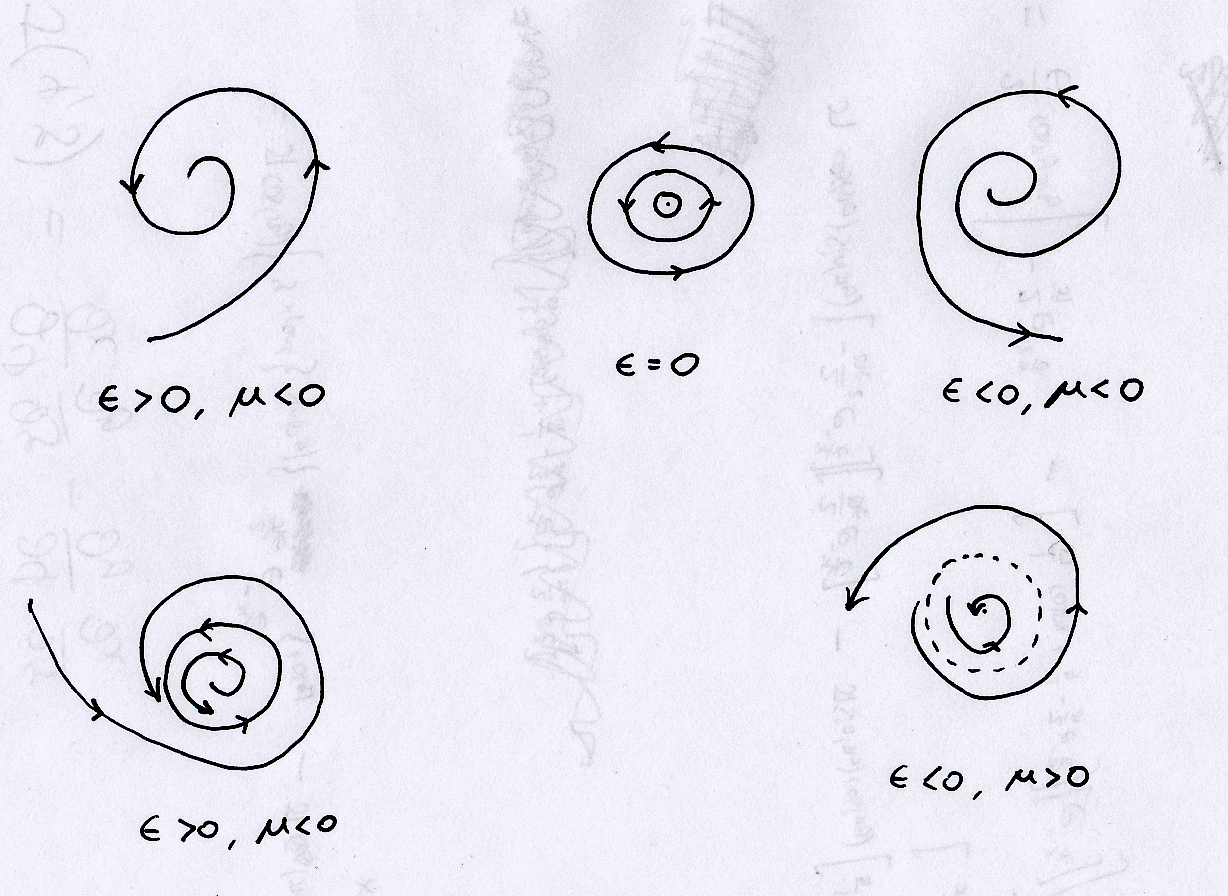
\includegraphics[width=8cm, height=6cm]{fig1.png}
\end{figure}
The infinite set of periodic solutions for $\epsilon = 0$ is destroyed by any 
perturbation to $\epsilon \neq 0$. This is an example of structural instability.
If $\mu > 0$ then just one limit cycle survives and is stable (unstable) for 
$\epsilon >0$ ($\epsilon < 0$). The appearance of the limit cycle as $\mu \uparrow$ 
through $0$ is another form of bifurcation.
\\
\\
\textbf{Example:} In 2D the points of successive interection $x_n$ of a 
solution near a limit cycle with a line $\varepsilon$ perpendicular to the cycle,
move monotonically towards/away from the point of intersection $x^{*}$ of 
$\varepsilon$ with the limit cycle.
% INSERT PLOT HERE
\begin{figure}[H]
\centering
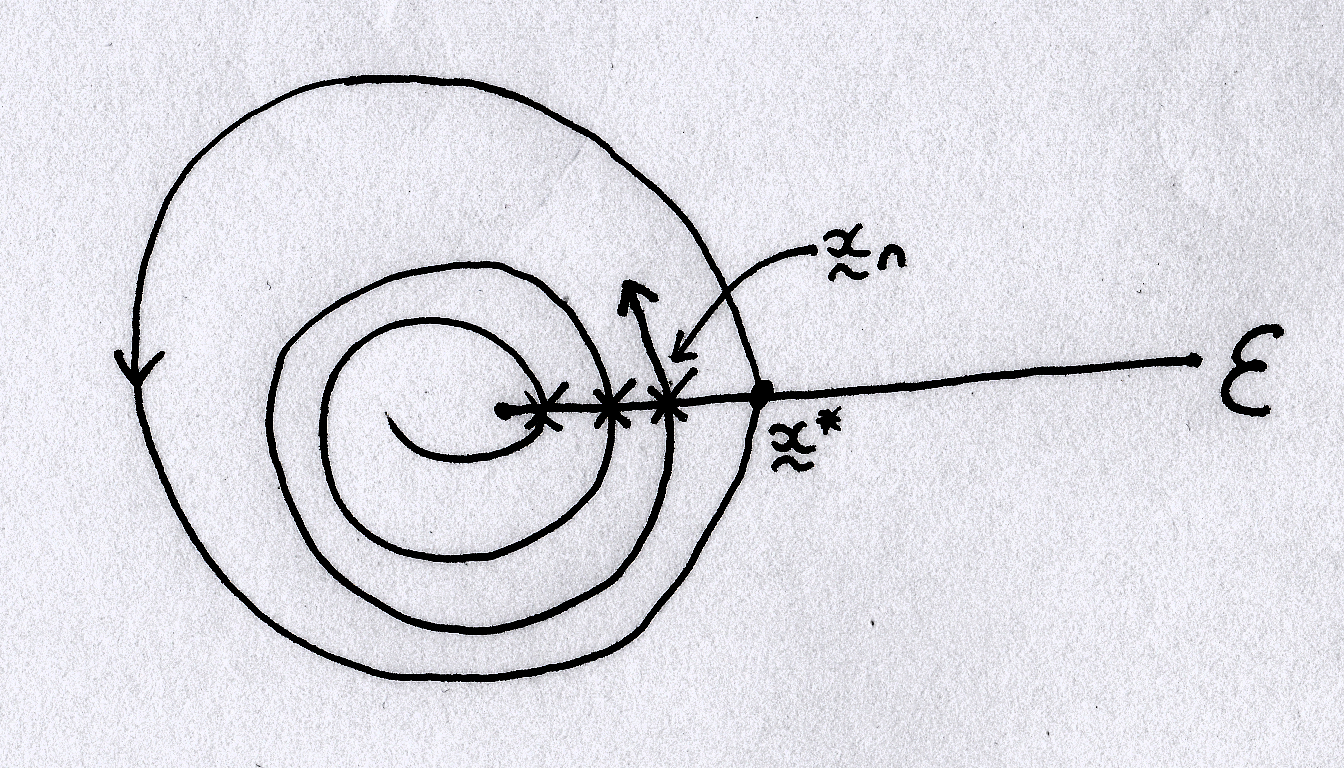
\includegraphics[width=7cm, height=4cm]{fig2.png}
\end{figure}
The point $x^{*}$ is a stable/unstable fixed point of this Poincar\'e recurrence
map.
\\
In 3 or higher dimensions, or in 2D with time-dependent coefficients there is 
room for much more complicated behaviour including \underline{chaos}.
%%%%%%%%%%%%%CHAPTER 1
\section{Basic Definitions}
We need some termonology.
\subsection{Notation}
We only consider ODEs of the form 
\begin{equation}\tag{*}
\dot{\textbf{x}} = \textbf{f(x)}
\end{equation}
for \textbf{x} in a phase space/state space $E \subset \mathbb{R}^{n}$.
The n first order ODEs form a dynamical system of order (dimension) n.
\\
\\
Since
\[ \frac{\partial \textbf{f} } { \partial t} = 0 \]
 we call the system \underline{autonomous}.
\\
\\
A non-autonomous system $\dot{\textbf{x}} = \textbf{f}(\textbf{x} ,t) $ can be
made autonomous by setting
\[ \textbf{y} = ( \textbf{x},t) \quad \mbox{ with } \quad \dot{\textbf{y}} = ( \textbf{f}(\textbf{y}),1) \]
The n$^{th}$ order ODE
\[ \frac{d ^n x}{d t^n} = g \left( x , \frac{d x}{d t} , \dots , \frac{d^{n-1} x}{d t^{n-1}} \right) \]
can be put in the form (*) by setting
\[ \textbf{y} =  \left( x , \frac{d x}{d t} , \dots , \frac{d^{n-1} x}{d t^{n-1}} \right) \]
with 
\[ \dot{\textbf{y}} =  \left( y_2 , y_3 , \dots , g( \textbf{y}) \right) \]
Similarly we will consider maps in the form
\[ \textbf{x}_{n+1} = \textbf{F}(\textbf{x}_n) \]
\subsection{Initial Value Problem}
Consider the IVP: 
\[ \dot{\textbf{x}} = \textbf{f}(\textbf{x})  \]
\[ \textbf{x}(t_0)  = \textbf{x}_0\]
In Analysis II we showed that if $\textbf{f}$ satisfies a Lipshitz condition
then we are guaranteed that a solution exists in a neighbourhood of $\textbf{x}_0$,
$ t_0$ and is unique.
\\
(Lipshitz condition is that $\exists$ $L$, $a$, s.t. 
$|\textbf{f}(\textbf{x})- \textbf{f}(\textbf{x})| < L|\textbf{x} - \textbf{y}|$
$, \quad \forall \; |\textbf{x}-\textbf{x}_0|, \; |\textbf{y}-\textbf{x}_0| < a$.)
\\
\\
Moreover, solutions $\textbf{x}(t \, ; \textbf{x}')$ to 
\[ \dot{\textbf{x}} = \textbf{f}(\textbf{x})  \]
\[ \textbf{x}(t_0)  = \textbf{x}'\]
exist, are unique and they depend continously on $\textbf{x}' , \, t$.
\\
\\
Note we are not guaranteed existence for all times.
\\
\\
\textbf{Example:} 
\[ \dot{x} = x^2  \]
\[ x(0)  = 1\]
This has solution
\[ x(t) = \frac{1}{1-t} \]
and so $x \to \infty$ as $t \uparrow 1$.
\\
\\
If $|\textbf{x}(t)| \to \infty$ as $t \to T \;(< \infty)$ then we call this
finite time blow up.
\\
\\
\textbf{Example:} Non-uniqueness when $\textbf{f}$ is non-Lipshitz. If
\[ \dot{x} = \left\{\begin{array}{lr}
				\sqrt{x} & \mbox{for } x >0 \\
				0        & \mbox{for } x \leq 0
				\end{array}
\right. \mbox{ and } x(0) = 0 \]
Then there is a family of solutions
\[ \left. \begin{array}{lr} 
				x = 0 & t < \tau \\
				x = \frac{1}{4}(t - \tau)^2 & t > \tau
\end{array} \right\} \mbox{ for any } \tau \geq 0 \]
From now on we will assume that \textbf{f} is differentiable ( and so Lipshitz).
\\
\subsection{Trajectories and Flows}
Consider the autonomous system
$ \dot{\textbf{x}} = \textbf{f}(\textbf{x}) $
The solution $\textbf{x}(t)$ to the IVP with $\textbf{x}(0) = \textbf{x}_0$
defines a trajectory. (orbit/integral curve)
\\
\\
The distance travelled along this curve clearly only depends on $t - t_0$, 
and we could consider lots of starting points $\textbf{x}_0$.
\\
This motivates the idea of a flow. 
\\
\\
\textbf{Definition:} (Flow) \\
Given \textbf{f}, the corresponding flow is defined to be a (the) function
$\bm{\phi}_t (\textbf{x}) $ from $E \times \mathbb{R} \to E$ such that
\[ 
\frac{\partial}{\partial t} \bm{\phi}_t ( \bm{x} ) = \bm{f}(\bm{\phi}_t (\bm{x} ) ), \qquad\
\bm{\phi}_0(\bm{x}) = \bm{x} 
 \]
The solution to the IVP $\dot{\bm{x}} = \bm{f}(\bm{x}), \; \bm{x}(t_0) = \bm{x}_0$,
is just $\bm{x}(t) = \bm{\phi}_{t - t_0} (\bm{x}_0)$
\\
Clearly 
\[ \bm{\phi}_{s+t}(\bm{x}) = \bm{\phi}_s(\bm{\phi}_t(\bm{x})) = \bm{\phi}_t ( \bm{\phi}_s (\bm{x} ) ) \]
\begin{framed}
\noindent Aside: We can establish another link with maps, by defining 
$\bm{x}_{n+1} = \bm{F}(\bm{x}_n) = \bm{\phi}_{\Delta t} (\bm{x}_n)$. \\
Clearly $\bm{\phi}_{n \Delta t} (\bm{x} ) = \bm{F} ( \bm{\phi}_{(n-1) \Delta t} (\bm{x} )) = \bm{F}^n(\bm{x}) $ 
\end{framed}
\subsection{Flows, Trajectories, Orbits, Invariant Sets, \& Limiting Sets}
Using the idea of a flow, we define the following:
\\
\\
\textbf{Definition:} Orbits/Trajectories
\\
 The orbit of $\bm{\phi}_t(\bm{x})$ through $\bm{x}_0$ is
the set $\mathcal{O}(\bm{x}_0) = \{ \bm{\phi}_t(\bm{x}_0): -\infty < t < \infty \}$.
\\
The forwards (backwards) orbit is 
\[\mathcal{O}^{+ \, (-)}(\bm{x}_0) = \{ \bm{\phi}_t(\bm{x}_0):  t \geq 0 \; (t \leq 0) \} \]
\textbf{Definition:} Invariant sets
\\
A set of points $\Lambda \subset E$ is invariant if
$\bm{x} \in \Lambda \implies \mathcal{O}(\bm{x}) \subset \Lambda$
\\
Clearly $\mathcal{O}(\bm{x}_0)$ is invariant, and so is any union of orbits.
\\
\\
Particular cases of interest are
\\
\\
\textbf{Definition:} Fixed points
\\
$\bm{x}_0$ is a periodic point with period $T$ if $\bm{\phi}_T(\bm{x}_0)= \bm{x}_0$
for some $T>0$ and $\bm{\phi}_t (\bm{x}_0) \neq \bm{x}_0$ for $0 < t < T$.
The set $ \{ \bm{\phi}_t ( \bm{x}_0) : 0 \leq t < T \}$ is the periodic orbit
through $\bm{x}_0$.
\\
\\
\textbf{Definition:} Limit Cycle
\\
A limit cycle is an isolated periodic orbit, i.e. there are no other periodic
orbits within a sufficiently small neighbourhood.
\\
\\
\textbf{Definition:} Homoclinic and Heteroclinic orbits
\\
If $\bm{x}_0$ is a fixed point and $\exists \; \bm{y} \neq \bm{x}_0$ such that
$\bm{\phi}_t(\bm{y}) \to \bm{x}_0$ as $t \to \pm \infty$ then 
$\mathcal{O}(\bm{y})$ is a homoclinic orbit.
\\
\\
If $\bm{x}_0$, $\bm{x}_1$ are fixed points and 
$\exists \; \bm{y} \neq \bm{x}_0 , \, \bm{x}_1$ with $\bm{\phi}_t (\bm{y}) \to \bm{x}_0$
as $t \to - \infty$, $\bm{\phi}_t(\bm{y}) \to \bm{x}_1$ as $t \to + \infty$ then
$\mathcal{O}(\bm{y})$ is a heteroclinic orbit.
%
\begin{figure}[H]
\centering\caption*{Example of a Heteroclinic and a Homoclinic orbit}
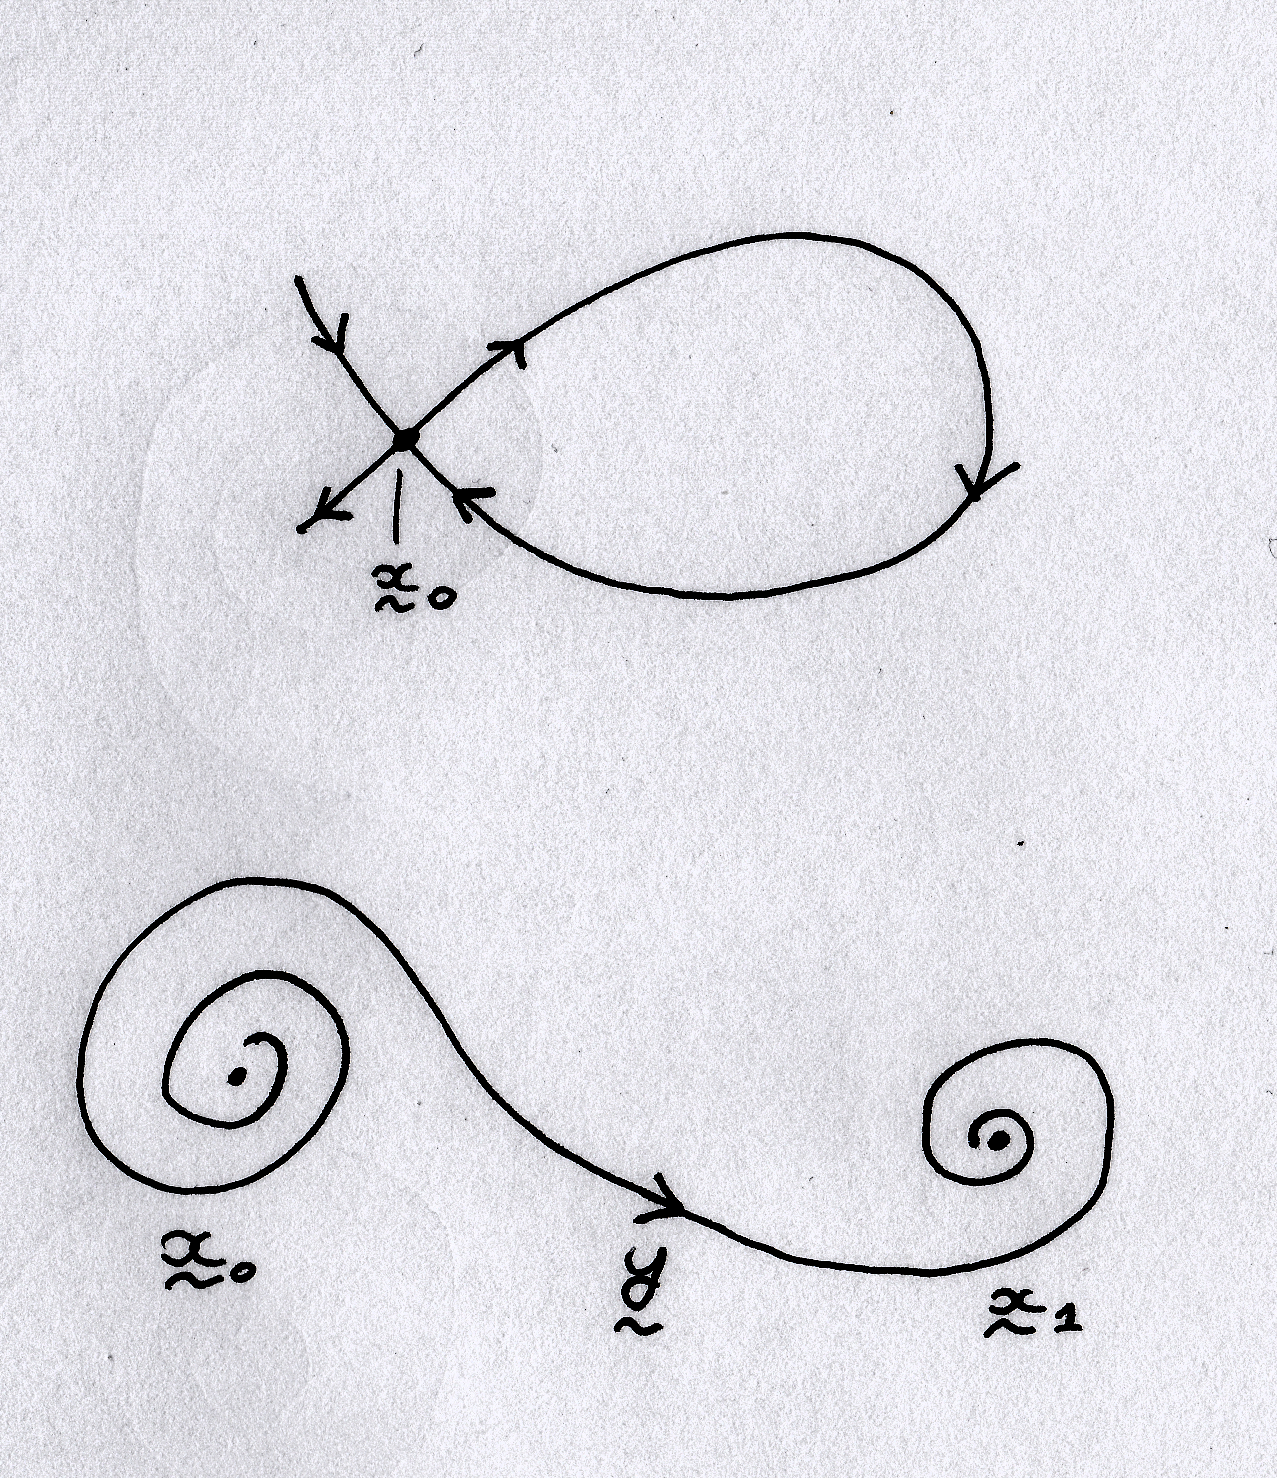
\includegraphics[width=4cm, height=6cm]{fig3.png}
\end{figure}
\noindent If we are interested in the long-term behaviour of trajectories, it is not 
enough simply to think of 
\[ \lim_{t \to \infty} \bm{\phi}_t(\bm{x}) \]
because the limit might not exist; for example a limit cycle.
\\
\\
\textbf{Definition:} Limit set
\\
The $\omega$-limit set of $\bm{x}$ is 
\[ \omega (\bm{x}) = \{ \bm{y} : \exists \mbox{ a sequence } (t_n) \mbox{ with }\
 \bm{\phi}_{t_n}(\bm{x}) \to \bm{y} \mbox{ and } t_n \to \infty \} \]
Similarly the $\alpha$ limit set is defined by sequences with $t_n \to - \infty$.
\\
\\
\textbf{Example:}
\begin{align*}
\dot{r} &= r(1-r^2) \\
\dot{\theta} &= 1
\end{align*}
\begin{figure}[H]
\centering
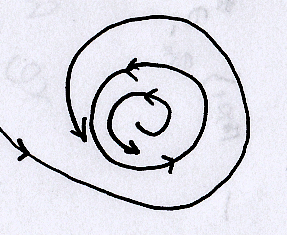
\includegraphics[width=2.5cm, height=2cm]{fig4.png}
\end{figure}
For $\bm{x}$ with $0 < |\bm{x}| < 1$ we have that
\[ \omega ( \bm{x} ) = \{ \bm{y} : |\bm{y}| = 1 \}  \qquad  \alpha ( \bm{x} ) = \{\bm{0} \} \]
For $|\bm{x}|>1$
\[ \omega ( \bm{x} ) = \{ \bm{y} : |\bm{y}| = 1 \}  \qquad  \alpha ( \bm{x} ) = \{ \} \]
\\
\\


\end{document}
